\documentclass[letterpaper,10pt]{article}

\usepackage{graphicx}                                        
\usepackage{amssymb}                                         
\usepackage{amsmath}                                         
\usepackage{amsthm}                                          

\usepackage{alltt}                                           
\usepackage{float}
\usepackage{color}
\usepackage{url}

\usepackage{balance}
\usepackage[TABBOTCAP, tight]{subfigure}
\usepackage{enumitem}
\usepackage{pstricks, pst-node}


\usepackage{geometry}
\geometry{textheight=8.5in, textwidth=6in}

\newcommand{\cred}[1]{{\color{red}#1}}
\newcommand{\cblue}[1]{{\color{blue}#1}}

\usepackage{hyperref}
\usepackage{geometry}

\def\name{Ryley Herrington}

%% The following metadata will show up in the PDF properties
\hypersetup{
  colorlinks = true,
  urlcolor = black,
  pdfauthor = {\name},
  pdfkeywords = {cs311 ``operating systems'' process control Unix},
  pdftitle = {CS 311 Project 2: UNIX Process Control},
  pdfsubject = {CS 311 Project 2},
  pdfpagemode = UseNone
}

\begin{document}
\begin{center}
{\large CS311 Project 2: Unix Process Control} \\ % \\ = new line
Ryley Herrington
February 3, 2012
\end{center}

\section{Introduction}
This project was supposed intended to read a text file, then output only the unique words in the file and the unique words would be printed out in alphabetical order, case insensitive   . It also uses the system sort command instead of figuring out how to compare chars to alphabetize the data. 

\section{Code Explanation}
Besides the comments in the code, this program might require some explanation. I made a series of utility functions to check and see if the creation of pipes and dup2 functions worked correctly and to close files and file descriptors. The only reason I did this is because we have a lot of those throughout the program. 

The method downcase str was made to go through every word and make it lower case before the sort happens. Then I pound define the maximum line length and maximum word length (200), and define read end to be 0, and write end to be 1. I do these define statements because it's easier to understand later. I create a connection type that has a pid, and two pipes for writing and reading and it initializes some values to -1 just in case I forget to later; it will throw errors unless I set it otherwise. 

The method to distribute words reads from an input stream and will distribute words (round robin style) to N output streams. The output streams will be tied to an external sorting process[es] , but this function doesn't deal with it because I will tie it manually. I run through every ascii character and if it's not an alpha character, I add it to the delimiter string. Then I go through the stream and tokenize the data into separate words, and at the same time I make them lowercase, and pass it to a file. The round robin portion is when I pass it to the current file modded by the amount of pipes. Finally we run a loop to close all of the file streams. It wasn't necessary to do it in this method, but it made it easier to understand. 

The method get word takes a FILE* and a char * and then uses frets to basically read a new word from the stream into a certain buffer. If it works it will fill the buffer and return 1, but when a stream is empty it will close the FILE* and free the buffer (returns 0). 

For merge words, I just implemented my own version of merge sort. For "W" words distributed across "F" files, we perform "F-1" comparisons times "W" words to be written. This might be improved by keeping the "current" words in  a more sophisticated structure (i.e. a sorted heap), but realistically, that would likely only matter for large N.  This is really for sorting data sets larger than memory, so the I/O time of getting the data probably dominates the comparison time in this merge.

It creates a one word butter for each input stream, and when the buffer is empty it will be deallocated and set to null to signify when the stream is empty. We run through to find the smallest word, and then we will compare rest of the words to find the smallest of the current set, then we write out the smallest token.  We do this over and over until every pipe is filled.

I created write streams and read streams by making a vector of FILE*'s and it would go through and write every word out, or read every word out depending on the method. And then return the stream to whatever functioned it. 

Wait for children just executes the waitpid function on each of the children (however many there were), and that's all. 

The parser creates the sorting processes and connect each with an input and output pipe. It creates the suppressor and connect a single pipe to it's input. Then reads stdin and distribute distinct words to each sorting process (round robin as aforementioned), merge sorts the results and then passes the date to the suppressor to eliminate duplicates. 

Basically, I have a for loop that runs through the amount of children we want, and then forks off and execs sort on the stream that is passed to the child. In the parent we close the correct sides of the pipe, and then we wait for the children.

 We also fork off an extra child  and exec suppressor which just fills two buffers with two of the next words from the sorter. It compares them and if they're the same it'll print out one but not the next one. Then it swaps buffers (last buff and curr buff), and loads in the next word.
 
 Finally back in uniqify.cpp we wait for the suppressor child to return and end the program.
\section{Revision Control Log}
\begin{table}[ht]
\caption{Revision Control Log} % title of Table
\centering  % used for centering table
\begin{tabular}{c c c c} % centered columns (4 columns)
\hline\hline                        %inserts double horizontal lines
Rev. \# & Date & Lines Changed & Description \\ [0.5ex] % inserts table 
%heading
\hline 
1.8 & 2/4 & +55 & Added final parsing method. Done. Added all comments. \\
1.7 & 2/3  & -21 + 8 & Added calls to suppressor and got rid of my other scanf function. \\ 
1.6 & 2/2 & -58 + 1 & Added suppressor file instead of inside uniqify.  \\
1.5 & 2/2 & + 44 & Added all comments, and added connection\_t and to\_lower function.  \\ 
1.4 & 2/1 & -21 + 8 & Added outline for suppressor,  got rid of extraneous get words method. \\
1.3 & 1/31 & -5 +9 & Rewrite to cpp, included vectors and removed all camelback identifiers. \\
1.2 & 1/31 & -18, +11 & Changed strtok to strsep, added error checking. \\
1.1 & 1/30 & +102 & Initial revision. \\[1.5ex] 
\hline
\end{tabular}
\label{table:nonlin} % is used to refer this table in the text
\end{table}


\section{Time Trials}
The time trials explained that the larger the file is, the longer it took to sort the data. This was expected, but I looked at the relationship between the size of the file and the time it took to sort. See graph:
\includegraphics[width=0.4\textwidth]{sz_vs_time.eps}


\end{document}
